\documentclass[12pt]{article}

%Begin----------------------------------------------------------------------------------------------------------------------------------------
%---------------------------------------------------------------------------------------------------------------------------------------------


%Package import and Config of Packages
%\usepackage[utf8]{inputenc}%\usepackage{tikz}#
\usepackage{lmodern}
\usepackage{setspace}
\usepackage{lastpage}
\usepackage{pgfplots} % Fuer Plots
\usepackage{pgfplotstable}
\usepackage{pgfkeys} 
\usepackage{filecontents}
\pgfplotsset{compat = newest}
\usepackage{tikz} % Generell gutes Packet
\usepackage{csvsimple} % Zum CSV auslesen
\usepackage{fancyhdr}
\usepackage{tcolorbox}


\usepackage[ngerman]{babel}
\usepackage{datetime}
\newdateformat{myformat}{\THEDAY{ten }\monthname[\THEMONTH], \THEYEAR}


\usepackage{subfig}
\usepackage{pdfpages}
\usepackage{subfiles}
\usepackage{titlesec}
\usepackage[pdfborder={0 0 0}]{hyperref}
\usepackage{pdfpages}
\usepackage{verbatim}
\usepackage{geometry}
\geometry{left=20mm, right=20mm, bottom=20mm}

\usepackage{graphicx}
\graphicspath{{../Bilder/}{Bilder/}}

\usepackage{xcolor}
\usepackage{listings}
%End------------------------------------------------------------------------------------------------------------------------------------------
%---------------------------------------------------------------------------------------------------------------------------------------------
%Package import and Config of Packages

%Begin----------------------------------------------------------------------------------------------------------------------------------------
%---------------------------------------------------------------------------------------------------------------------------------------------
%List Configuration for Coding
\usepackage{listings} % Generell Code-Boxen
\usepackage{xcolor} % Fuer extra Farben mit color{}

\colorlet{punct}{red!60!black}
\definecolor{background}{HTML}{EEEEEE}
\definecolor{delim}{RGB}{20,105,176}
\colorlet{numb}{magenta!60!black}

\definecolor{mGreen}{rgb}{0,0.6,0}
\definecolor{mGray}{rgb}{0.5,0.5,0.5}
\definecolor{mPurple}{rgb}{0.58,0,0.82}
\definecolor{backgroundColour}{rgb}{255,255,255}
\lstdefinestyle{CStyle}
{
    backgroundcolor=\color{backgroundColour},   
    frame=single,
    belowcaptionskip=1\baselineskip,
    breaklines=true,
    xleftmargin=\parindent,
    language=C,
    showstringspaces=false,
    basicstyle=\footnotesize\ttfamily,
    keywordstyle=\bfseries\color{magenta},
    commentstyle=\color{mGreen},
    identifierstyle=\color{blue},
    stringstyle=\color{orange},
}   

%End------------------------------------------------------------------------------------------------------------------------------------------
%---------------------------------------------------------------------------------------------------------------------------------------------
%List Configuration for Coding


%Begin----------------------------------------------------------------------------------------------------------------------------------------
%---------------------------------------------------------------------------------------------------------------------------------------------
%More Subsections Configuration
\titleclass{\subsubsubsection}{straight}[\subsection]
\newcounter{subsubsubsection}[subsubsection]
\renewcommand\thesubsubsubsection{\thesubsubsection.\arabic{subsubsubsection}}
\renewcommand\theparagraph{\thesubsubsubsection.\arabic{paragraph}} % optional; useful if paragraphs are to be numbered
\titleformat{\subsubsubsection}
  {\normalfont\normalsize\bfseries}{\thesubsubsubsection}{1em}{}
\titlespacing*{\subsubsubsection}
{0pt}{3.25ex plus 1ex minus .2ex}{1.5ex plus .2ex}


\titleclass{\subsubsubsubsection}{straight}[\subsection]
\newcounter{subsubsubsubsection}[subsubsubsection]
\renewcommand\thesubsubsubsubsection{\thesubsubsubsection.\arabic{subsubsubsubsection}}
\titleformat{\subsubsubsubsection}
  {\normalfont\normalsize\bfseries}{\thesubsubsubsubsection}{1em}{}
\titlespacing*{\subsubsubsubsection}
{0pt}{3.25ex plus 1ex minus .2ex}{1.5ex plus .2ex}

\makeatletter
\renewcommand\paragraph{\@startsection{paragraph}{5}{\z@}%
  {3.25ex \@plus1ex \@minus.2ex}%
  {-1em}%
  {\normalfont\normalsize\bfseries}}
\renewcommand\subparagraph{\@startsection{subparagraph}{6}{\parindent}%
  {3.25ex \@plus1ex \@minus .2ex}%
  {-1em}%
  {\normalfont\normalsize\bfseries}}
\def\toclevel@subsubsubsection{4}
\def\toclevel@paragraph{5}
\def\toclevel@paragraph{6}
\def\l@subsubsubsection{\@dottedtocline{4}{7em}{4em}}
\def\l@subsubsubsubsection{\@dottedtocline{5}{8em}{5em}}
\def\l@paragraph{\@dottedtocline{5}{10em}{5em}}
\def\l@subparagraph{\@dottedtocline{6}{14em}{6em}}
\makeatother

\setcounter{secnumdepth}{5}
\setcounter{tocdepth}{5}

%End------------------------------------------------------------------------------------------------------------------------------------------
%---------------------------------------------------------------------------------------------------------------------------------------------
%More Subsections Configuration


\pagestyle{fancy}
\fancyhf{}


%Begin----------------------------------------------------------------------------------------------------------------------------------------
%---------------------------------------------------------------------------------------------------------------------------------------------
%TitelSeite
\title{DIC-Serielle Kommunikation mit einem µC 
}
\author{Fabio~Plunser}
\date{\today}
\rhead{\hspace{5px}
\includegraphics[scale=0.09]{Bilder/logo.png}}
\lhead{DIC-Serielle Kommunikation mit einem µC}
\rfoot{Page~\thepage ~of~\pageref{LastPage}}
\lfoot{PlunserFabio}
\renewcommand{\headrulewidth}{1pt}
\renewcommand{\footrulewidth}{1pt}



\begin{document}
\pagenumbering{gobble}

\begin{titlepage}
  \maketitle
  \begin{figure}[!htb]
    \centering
    \includegraphics[scale=1]{UART-TitelBild.png}
    \label{UART-TitelBild}
  \end{figure}
  
\end{titlepage}

%End------------------------------------------------------------------------------------------------------------------------------------------
%---------------------------------------------------------------------------------------------------------------------------------------------
%TitelSeite

%Begin----------------------------------------------------------------------------------------------------------------------------------------
%---------------------------------------------------------------------------------------------------------------------------------------------
%Inhaltsverzeichnis
\pagebreak
\thispagestyle{empty}
\renewcommand\contentsname{Inhaltsverzeichnis}
\tableofcontents	
\pagenumbering{gobble}

%End------------------------------------------------------------------------------------------------------------------------------------------
%---------------------------------------------------------------------------------------------------------------------------------------------
%Inhaltsverzeichnis

%Begin----------------------------------------------------------------------------------------------------------------------------------------
%---------------------------------------------------------------------------------------------------------------------------------------------
%Abbildungsverzeichnis
\thispagestyle{empty}
\renewcommand\listfigurename{Abbildungsverzeichnis}
\listoffigures
%End------------------------------------------------------------------------------------------------------------------------------------------
%---------------------------------------------------------------------------------------------------------------------------------------------
%Abbildungsverzeichnis
\renewcommand\lstlistlistingname{Code}
\lstlistoflistings

%Begin----------------------------------------------------------------------------------------------------------------------------------------
%---------------------------------------------------------------------------------------------------------------------------------------------
%Codeverzeichnis
% \renewcommand\lstlistlistingname{Codeverzeichnis}
% \lstlistoflistings
\pagebreak
\pagenumbering{arabic}

%End------------------------------------------------------------------------------------------------------------------------------------------
%---------------------------------------------------------------------------------------------------------------------------------------------
%Codeverzeichnis



%Begin----------------------------------------------------------------------------------------------------------------------------------------
%---------------------------------------------------------------------------------------------------------------------------------------------
%Main
\newpage
\section{Aufgabenstellung}
    Die Aufgabe ist es auf dem STM32F030F4 Chip die UART3 so zu programmieren, dass sie den Wert eines eingebauten ADC per interrupt ausgibt.\\
    Die richtige Aufgabe ist es die STM32F030F4 UART3 zu programmieren dass sie wenn sie ein zeichen erhält 10 Bytes zurückschickt. \\
    Da dieses spezielle Package des STM32 keine UART3 besitzt ist die Aufgabenstellung so nicht möglich somit wird einfach die vorhandene UART1 Schnittstelle verwendet.\\
    Der STM UART Ausgang wird mit einem MAX485 auf RS485 übersetzt.\\
    UART einstellungen:\\
    Baudrate: 38400 mit ODD parity\\\\
    
    \noindent Dieser Arbeitsauftrag kann in dieser GIT-Repo verfolgt werden: \url{https://github.com/FabioPlunser/DIC-Lezuo}
    


\newpage
\section{RS485}
    \subsection{Generelles}
        Ist ein Industriestandard der eine asynchrone serielle Datenübertragung ermöglicht. \\
        Der Standard verwendet ein symmetrisches Leitungspaar, dass für eine höhere elektromagnetische Resistenz sorgt.\\\\

    \subsection{Wie funktioniert es?}
        Betriebsspannung 5V oder 3.3V\\
        Der empfänger wertet die die Differenz beider Leitungen aus und kann Pegel ab $\pm 200mV$ erkennen.\\
        Senderpegel können von $\pm 1.5V bis \pm 6V$\\
        Logik: \\
        Wenn $U_{+} - U_{-} < -0.3V$ = MARK = OFF = Logisch 1\\
        Wenn $U_{+} - U_{-} > +0.3V$ = SPACE = ON = Logisch 0 \\


        \begin{figure}[!htb]
            \centering
            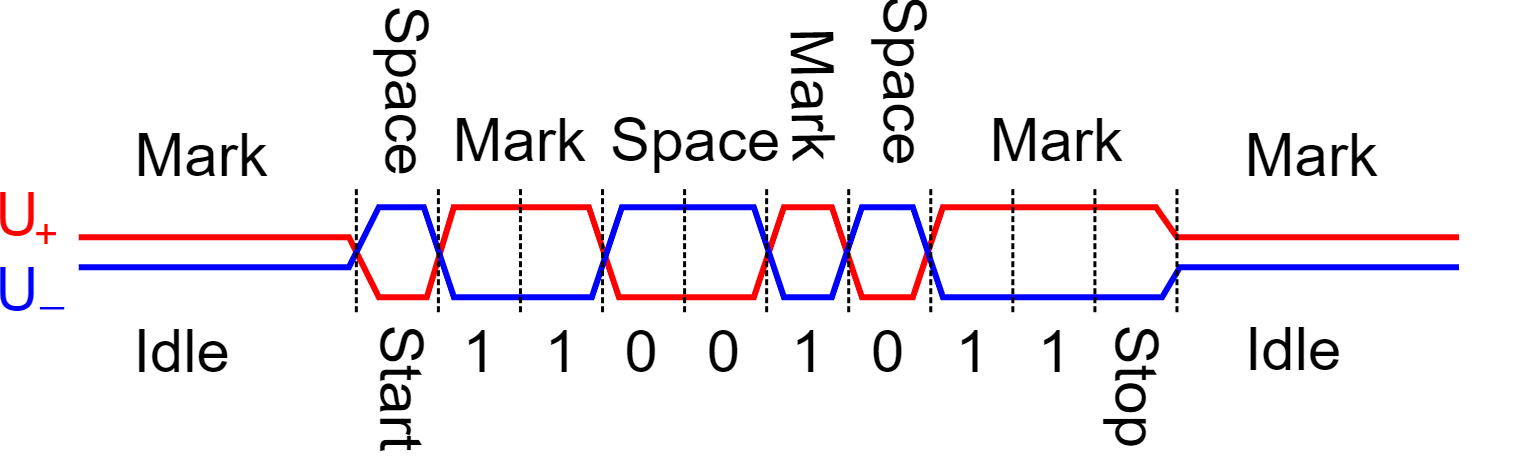
\includegraphics[scale=0.45]{RS485-Diagramm.png}
            \caption{RS485-Diagramm}
            \label{caption:RS485-Diagramm}
        \end{figure}
        

\newpage
    \subsection{Wie wird der MAX485 angeschlossen}
        
        Unten ist ein Beispiel mit einem Arduino UNO\\
        Anschluss:\\
        DI $\rightarrow$ TX\\
        RO $\rightarrow$ RX\\
        DE, RE auf einen GPIO Pin. Da wenn DE + RE = 1 $\rightarrow$ Daten können nur gesendet werden.\\
        Wenn DE + RE = 0 $\rightarrow$ Daten können nur empfangen werden.\\\\
    
        \begin{figure}[!htb]
            \centering
            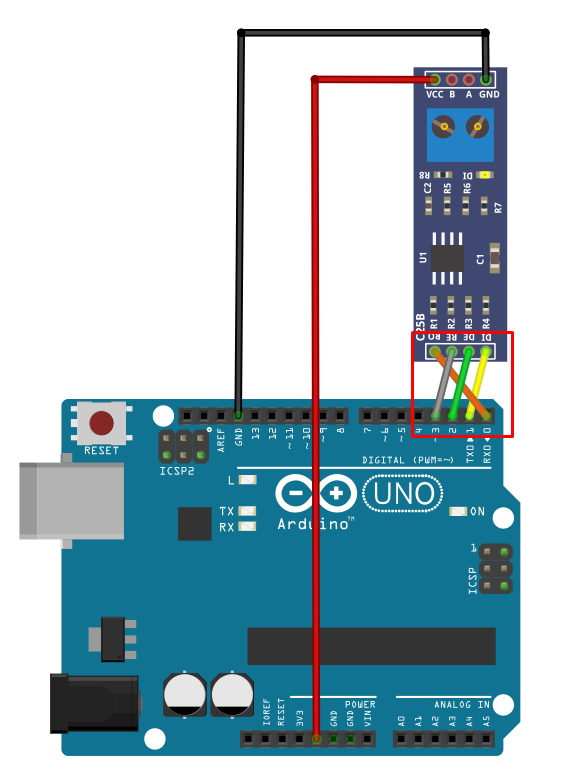
\includegraphics[scale=0.5]{MAX485-Arduino-Anschluss-BSP.png}
            \caption{MAX485-Arduino-Anschluss-BSP}
            \label{caption:MAX485-Arduino-Anschluss-BSP}
        \end{figure}

\newpage
        \noindent Ebenso muss dann der MAX485 and dem STM angeschlossen werden. Das untere Bild ist das Demo Board des STM32F030F4, eines der wenigen Boards, dass man zum Testen des Programmes 
        für den STM Chip kaufen kann.
    
        \begin{figure}[!htb]
            \centering
            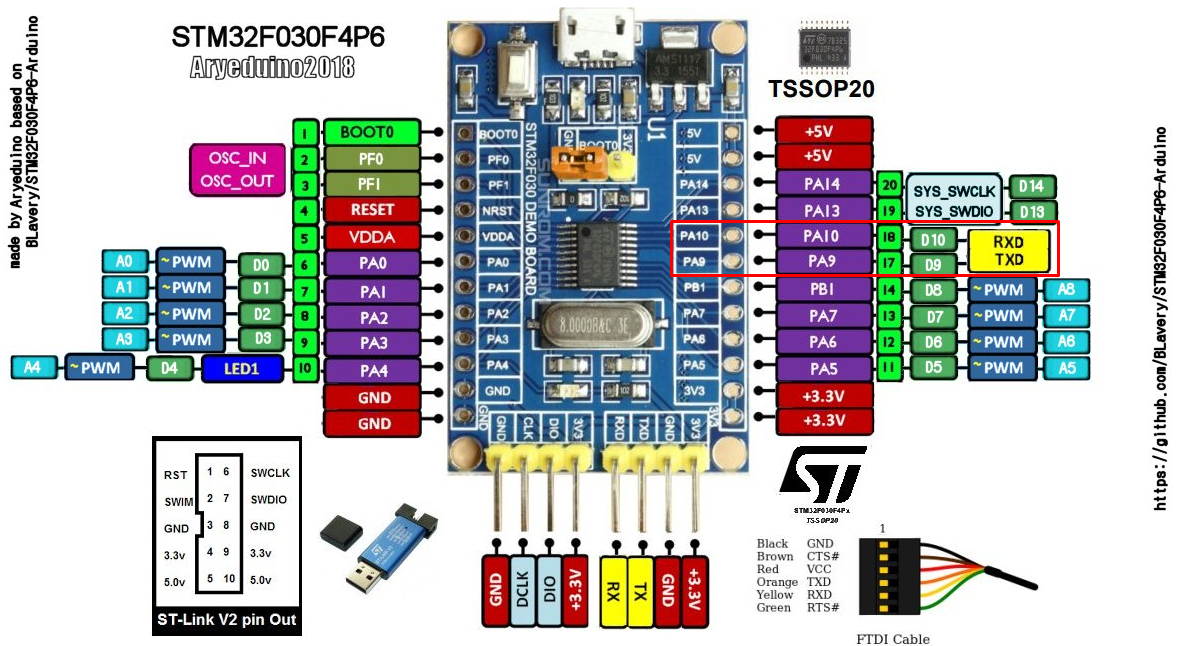
\includegraphics[scale=0.5]{STM32F030F4P6-Pinout.png}
            \caption{STM32F030F4P6-Pinout}
            \label{caption:STM32F030F4P6-Pinout}
        \end{figure} 
        
\newpage
\section{Einteilung | Was man wissen muss}
    \begin{itemize}
        \item Clock aufbau / einstellen
        \item GPIO Pins register finden / GPIO Pins einstellen 
        \item UART Register suchen / UART aktivieren und einstellen
        \item Verstehen wie NVIC funktioniert
    \end{itemize}

\newpage
\section{Clock}
    Die Clock wird am einfachsten, passend aus der gewollten Baudrate für die USART ausgewählt. Damit die Baudrate richtig berechnet wird.\\
    Die HSI Clock von 8MHz ist standard mäßig aktiviert.\\
    Weiterhin werden im APB2 Bus die Clocks für die USART1 und für den ADC und im AHB Bus für die GPIO Ports aktiviert. 
    Die weiteren Clock einstellungen wie z.B. für die USART sind in der jeweilign Initiallisierungs Funktion enthalten.
    
    \begin{figure}[!htb]
        \centering
        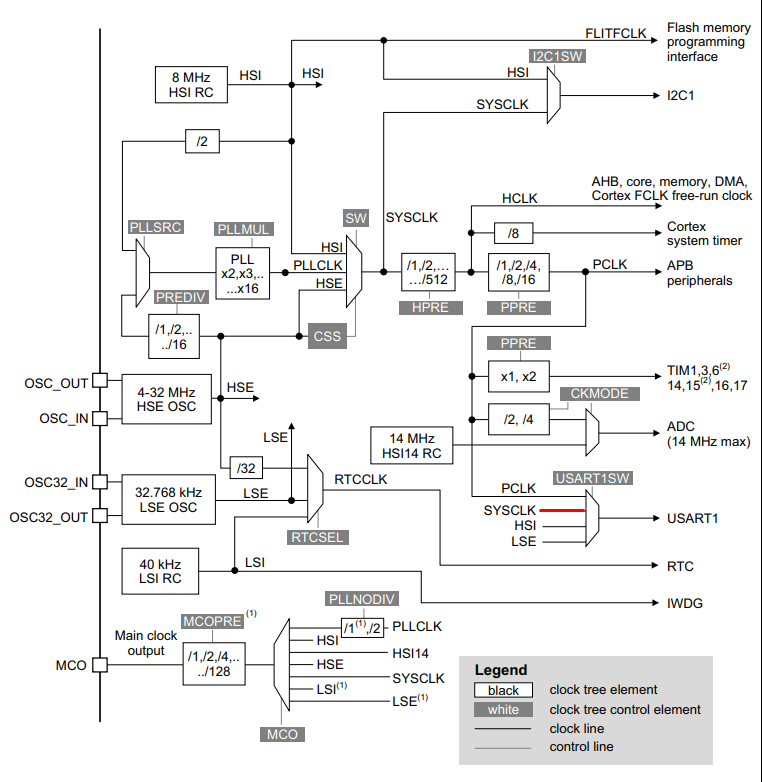
\includegraphics[scale=0.65]{Clock-Tree.png}
        \caption{Clock-Tree}
        \label{caption:Clock-Tree}
    \end{figure}
    
    
\newpage
\subsection{Clock-Code}
\begin{lstlisting}[language=C, style=CStyle, caption=init-CLOCK, captionpos=b, label=init-CLOCK]
int init_CLOCK()
{
    uint32_t reg_content;
    uint32_t* rcc_ahbenr = RCC_AHBENR; 
    uint32_t* rcc_apb2enr = RCC_APB2ENR;
    uint32_t* rcc_cfgr = RCC_CFGR;

    //GPIO A port clock enable
    reg_content = *rcc_ahbenr;
    reg_content |= 0x00020000;
    *rcc_ahbenr = reg_content;
    
    //USART1 clock enable
    reg_content = *rcc_apb2enr;
    reg_content |= 0x00004200;
    *rcc_apb2enr = reg_content;

    //set AHB Clock to not divided so same clock as sysclock
    reg_content = *rcc_cfgr;
    reg_content |= 0x00000000;
    *rcc_cfgr = reg_content; 
}
\end{lstlisting}
\newpage
\section{GPIO}
    \subsection{GPIO-Erklärung}
    Wie man bei der Abbildung \ref{caption:System-Architektur} sehen kann, sind die GPIOs am BUS AHB2 verbunden. 
    Da das verwendete Paket nur GPIO A verwendet müssen dementsprechend die GPIO-A Register richtig konfiguriert werden\\
    Das Register um die GPIOs als output einzustellen ist \textbf{GPIOA\_MODER im Addressraum 0x4800 0000 (des AHB2 Buses) mit dem Address offset: 0x00}\\
    Um Pins für die UART verwenden zu können müssen diese Pins noch als $"$alternate functions$"$ konfiguriert werden im Register \textbf{GPIOA\_AFRH mit Address offset: 0x24}.
    Welche Pin Nummer man Programmieren muss, sieht man in der Abbildung \ref{caption:GPIO-UART-PIN-Table}, man benötigt PA9 (Pin:17) und PA10 (Pin:18), da diese als alternate function
    die USART\_1 TX und RX hinterlegt haben. Wie das alternate function Register konfiguriert werden muss sieht man in den Abbildungen \ref{caption:GPIO-AF} 
    und \ref{caption:GPIO-AF-Register}\\\\
    Weiterhin müssen noch zwei GPIO Pins Für die DE und RE Pins des MAX485 als output konfiguriert werden. Ich verwend PA7 und PA8.\\
    Ebenfalls wird ein GPIO Pin als analog konfiguriert um diesen als ADC Eingang zu verwenden. 
    

    \begin{figure}[!htb]
        \centering
        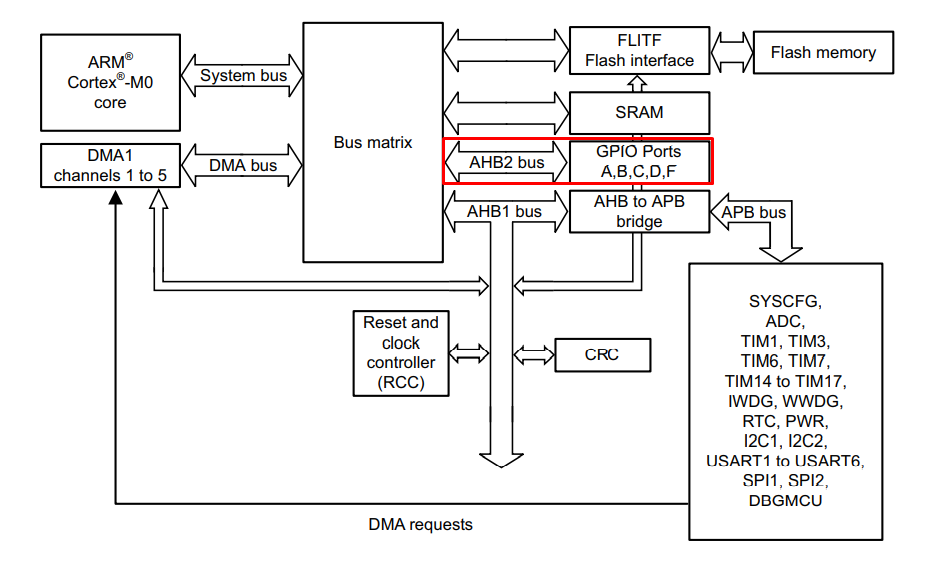
\includegraphics[width=\linewidth]{System-Architektur.png}
        \caption{System-Architektur}
        \label{caption:System-Architektur}
    \end{figure}

\newpage
    \begin{figure}[!htb]
        \centering
        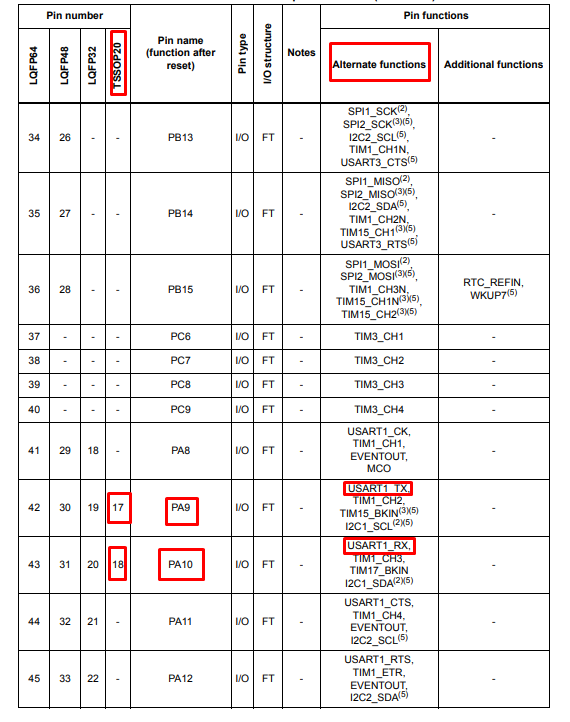
\includegraphics[scale=0.90]{GPIO-UART-PIN-Table.png}
        \caption{GPIO-UART-PIN-Table}
        \label{caption:GPIO-UART-PIN-Table}
    \end{figure}

\newpage
    \begin{figure}[!htb]
        \centering
        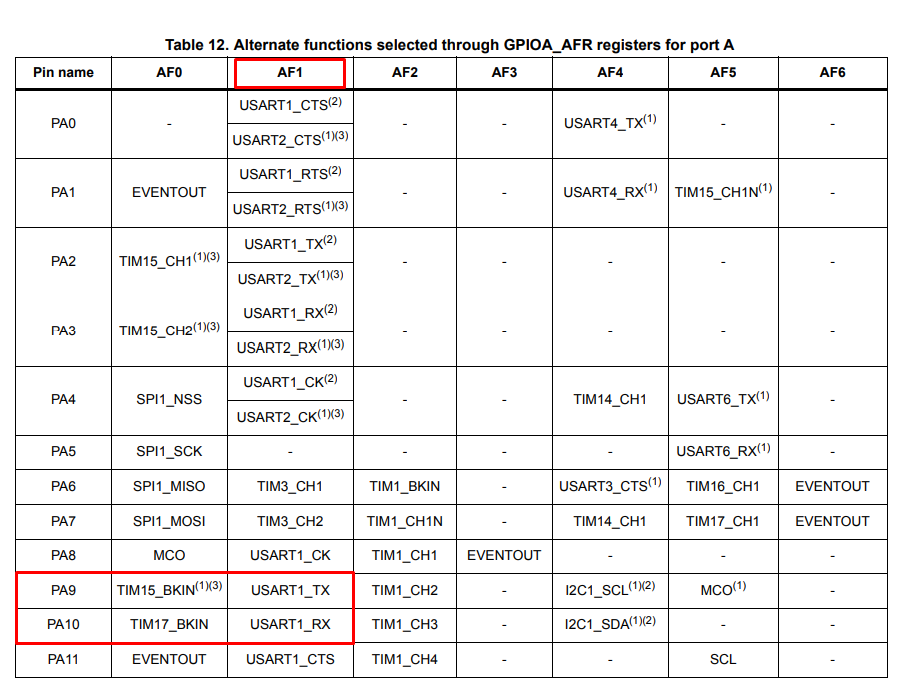
\includegraphics[scale=0.65]{GPIO-AF.png}
        \caption{GPIO-AF}
        \label{caption:GPIO-AF}
    \end{figure}
    
\newpage
    \begin{figure}[!htb]
        \centering
        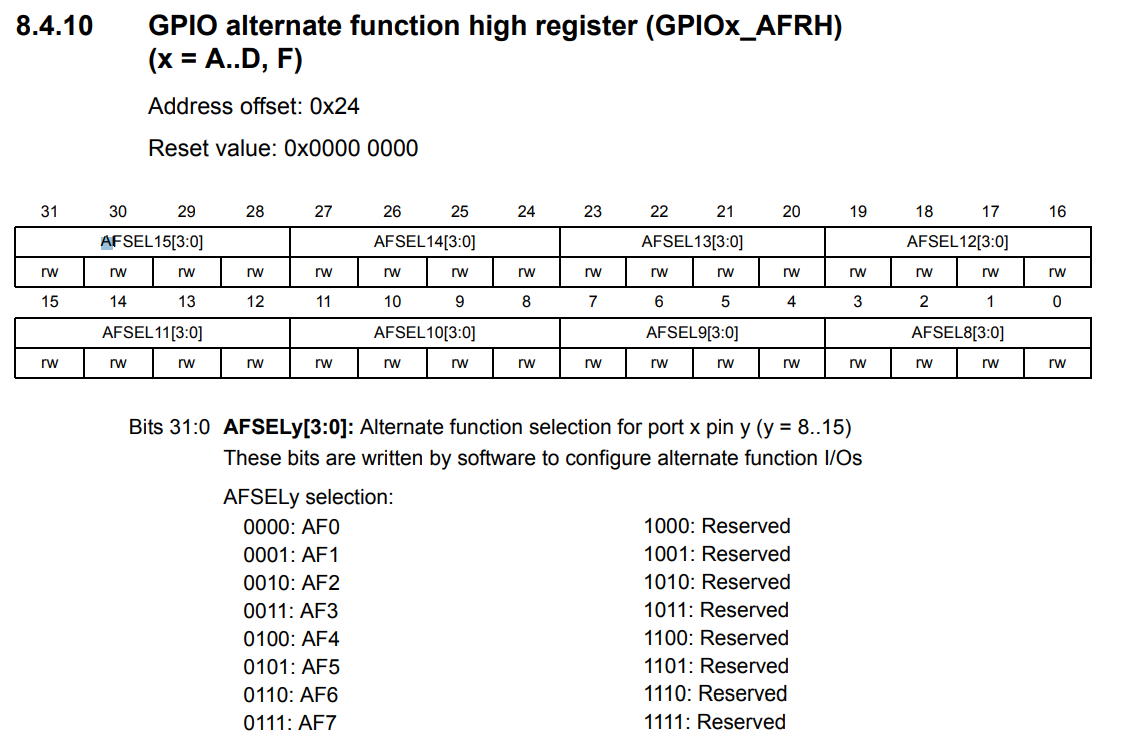
\includegraphics[scale=0.65]{GPIO-Alternate-function.png}
        \caption{GPIO-AF-Register}
        \label{caption:GPIO-AF-Register}
    \end{figure}
        
\newpage
\subsection{GPIO-Code}
    \begin{lstlisting}[language=C, style=CStyle, caption=GPIO-Code, captionpos=b, label=GPIO-Code]
int init_GPIO()
{
    //Set GPIO pins PA9 and PA10 alternate function for USART TX and RX, 
    //set PA7 and PA6 output for DE and RE of MAX485 
    //PA0 ADC_IN0 so set it to analog and then in DAC register set PA0 as ADC_IN0 
    uint32_t reg_content;
    uint32_t* gpioa_moder = GPIOA_MODER;
    uint32_t* gpioa_afrh = GPIOA_AFRH;
    uint32_t* gpioa_odr = GPIOA_ODR;

    reg_content = *gpioa_moder;
    reg_content |= 0x00285003;
    *gpioa_moder = reg_content;

    //Set GPIO PA9 as AF=TX and PA10 as AF = RX
    reg_content = *gpioa_afrh;
    reg_content |= 0x00000110;
    *gpioa_afrh = reg_content;

    //Ensure that output gpios are 0 for MAX, to read all the time
    //and only send, when needing to send
    reg_content = *gpioa_odr;
    reg_content |= 0x00000000;
    *gpioa_odr = reg_content;  
}
    \end{lstlisting}
        
    
    
    
    % \begin{figure}[!htb]
    %     \centering
    %     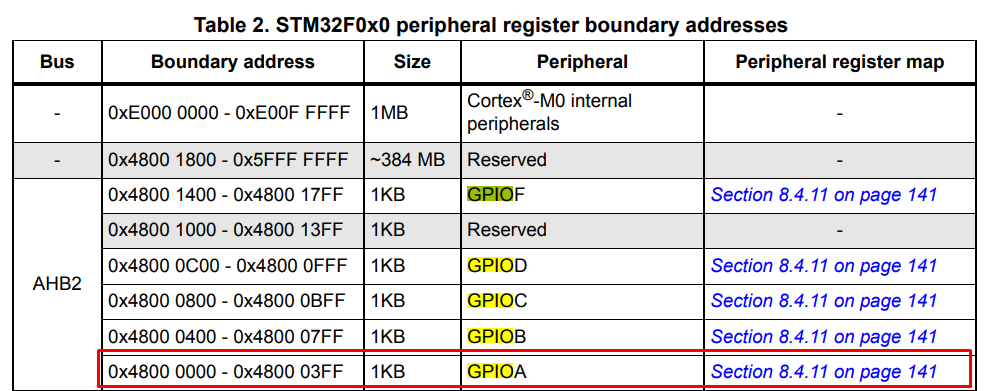
\includegraphics[scale=1]{GPIO-A-Boundary-address.png}
    %     \caption{GPIO-A-Boundary-address}
    %     \label{caption:GPIO-A-Boundary-address}
    % \end{figure}


    % \begin{figure}[!htb]
    %     \centering
    %     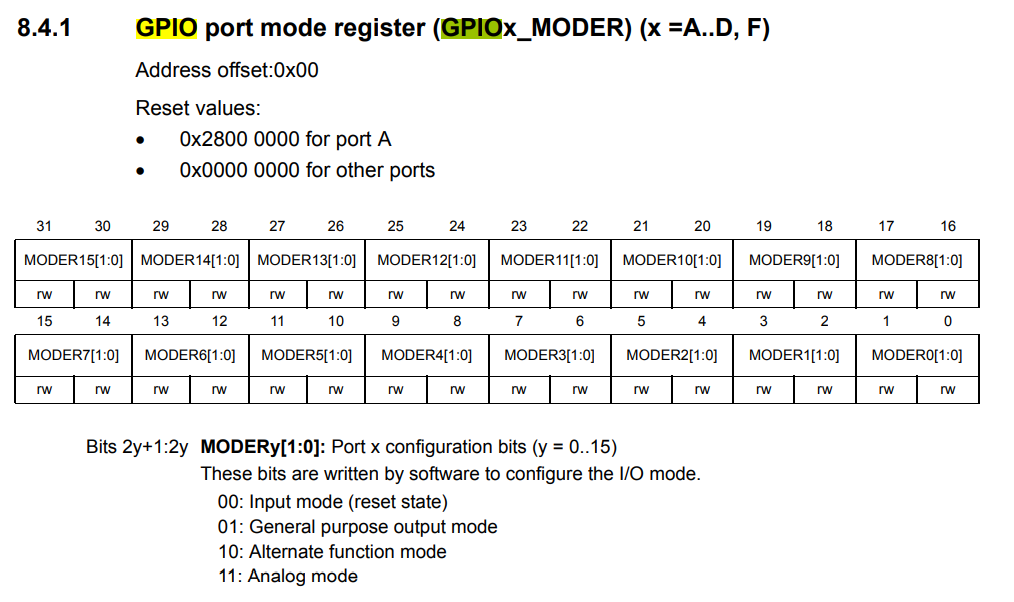
\includegraphics[scale=1]{GPIOx-Register.png}
    %     \caption{GPIOx-Register}
    %     \label{caption:GPIOx-Register}
    % \end{figure}


    

\section{USART}
    USART Addressraum:  \textbf{0x4001 3800 - 0x4001 3BFF}
    Für die USART muss, die Clock, die Bautrate, Parity, Wordlenght und die Interrupts eingestellt werden. 
    \subsection{Baudrate-Berechnung-Register-Setzen}
        Um die Baudrate einstellen zu können muss in das Register \textbf{USART\_BRR} die richtige Hexadezimal Zahl geschrieben werden.\\\\
        Berechnung: $\frac{Clock}{Baudrate}$, $\frac{8MHz}{38400}$ = 208,3$_{dezimal}$ bzw. D0$_{hex}$\\
        Zurückgerechnet $208*38400 = 7.98MHz. \frac{8MHz}{208} = $Baudrate von $38461$.\\\\
        Da der Systemclock gleich der HSI clock ist, kann dafür im Register \textbf{RCC\_CFGR3 bei der Addresse offset: 0x30} die USART1SW entweder 
        mit $01$ für Systemclock oder mit $11$ für HSI clock beschrieben werden. Zusätzlich muss im Register \textbf{USART\_BRR mit Address offset: 0x0C} D0 geschrieben
        Werden.
        
        \begin{figure}[!htb]
            \centering
            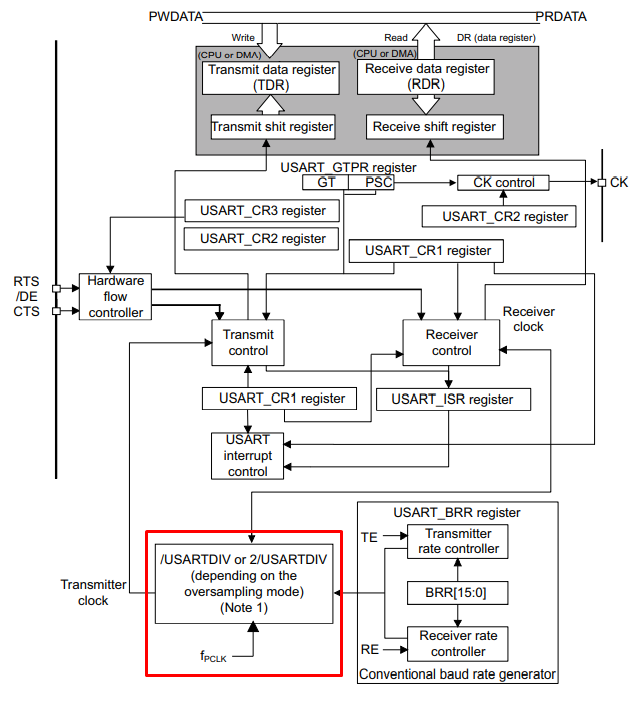
\includegraphics[scale=0.50]{USART-Aufbaug.png}
            \caption{USART-Aufbaug}
            \label{caption:USART-Aufbaug}
        \end{figure}
        \begin{figure}[!htb]
            \centering
            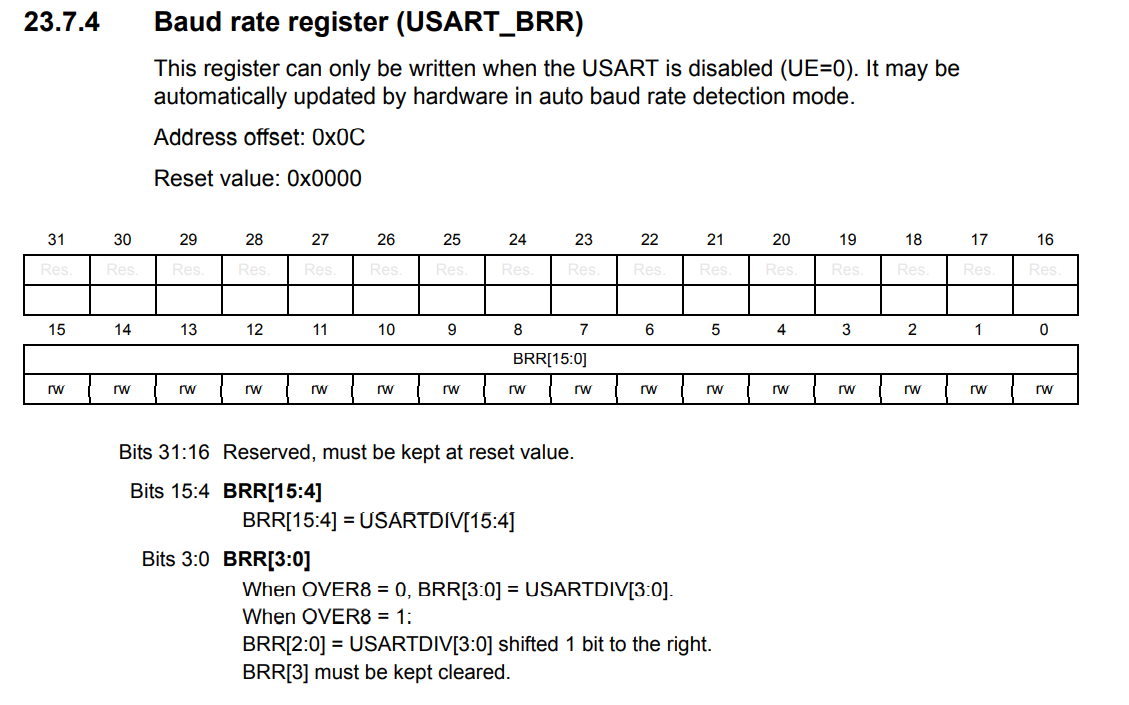
\includegraphics[scale=0.45]{USART-BRR.png}
            \caption{USART\_BRR}
            \label{caption:USART-BRR}
        \end{figure}
      
\newpage
    \subsection{Weitere USART einstellungen}
        Die Eistellungen der USART müssen getroffen werden, bevor sie aktiviert wird. Laut angabe wird noch eine ODD Parity verwendet diese kann in dem Register
        \textbf{USART\_CR1} auf Bit9: festgelegt werden. Weiterhin müssen dort unter Bit3 und Bit2, TX und RX aktivieren.

    \subsection{USART-Initiallisierung/Konfiguration|Code}
        \begin{lstlisting}[language=C, style=CStyle, caption=Init-UART, captionpos=b, label=Init-UART]
int init_UART()
{   
    uint32_t reg_content;
    uint32_t* rcc_cfr3 = RCC_CFGR3;
    uint32_t* usart1_brr = USART1_BRR;
    uint32_t* usart1_cr1 = USART1_CR1;

    //Use SYSCLK for USART and use Baudrate 38400
    reg_content = *rcc_cfr3;                
    reg_content |= 0x00000001;
    *rcc_cfr3 = reg_content; 
    
    reg_content = *usart1_brr;
    reg_content = 0x00000D00;
    *usart1_brr = reg_content;
    
    //Wordlenght, Parity control enable, Parity selection, interrupt enable, Transmission complete interrupt enable, RXNE interrupt enable
    reg_content = *usart1_cr1;
    reg_content |= 0x000006EC;
    *usart1_cr1 = reg_content;

    reg_content = *usart1_cr1;
    reg_content |= 0x00000001; //enable UART
    *usart1_cr1 = reg_content;
}
        \end{lstlisting}
        
    \subsection{USART-InterruptHandler}
    \begin{lstlisting}[language=C, style=CStyle, caption=Init-UART, captionpos=b, label=Init-UART]
void USART1_IRQHandler(void)
{   
    uint32_t* usart1_isr = USART1_ISR;
    uint32_t usart1_isr_rxne = USART1_ISR_RXNE;
    uint32_t usart1_isr_tc = USART1_ISR_TC;
    uint32_t* usart1_tc = USART1_ICR;
    uint32_t* usart1_tc_tcce = USART1_ICR_TCCF;
    uint32_t* usart1_tdr =  USART1_TDR;
    uint32_t* gpioa_odr = GPIOA_ODR;
    uint32_t reg_content;

    if ((*usart1_isr & usart1_isr_tc) == usart1_isr_tc)
    {
        if (send == sizeof(USART_write_data)) 
        {
            //set MAX to listen 
            reg_content = *gpioa_odr;
            reg_content |= 0x00000000;
            *gpioa_odr = reg_content;          
            send=0;
            *usart1_tc |= *usart1_tc_tcce; // Clear transfer complete flag *      
        }
        else
        {
            // clear transfer complete flag and fill TDR with a new char 
            *usart1_tdr = USART_write_data[send++];
        }
    }

    //when something comes at usart, begin to write the ADC Data 
    if ((*usart1_isr & usart1_isr_rxne) == usart1_isr_rxne)
    {
        USART_READ = *((char *)USART1_RDR);
        //Set PA7 and PA6 high for max to send data
        reg_content = *gpioa_odr;
        reg_content |= 0x000000C0;
        *gpioa_odr = reg_content;

        *usart1_tdr  = USART_write_data[0];
    }
}
    \end{lstlisting}
                

    
   
\newpage
\section{ADC}
    \subsection{Erklärung}
    Der STM hat einen ADC eingebaut, dieser kann bei den größeren Packages sogar als Temperatursensor verwendet werden.
    Alle GPIOs können als ADC Eingang verwendet werden solange sie als analog GPIO konfiguriert werden. 
    
    \subsection{Register}
        Die Register für den ADC beginnen bei 0x4001 2400 bis 0x4001 27FF.
        Für die Konfiguration werden folgende Register benötigt:

        \subsubsection{ADC\_ISR | ADC Interrupts}
            \begin{figure}[!htb]
                \centering
                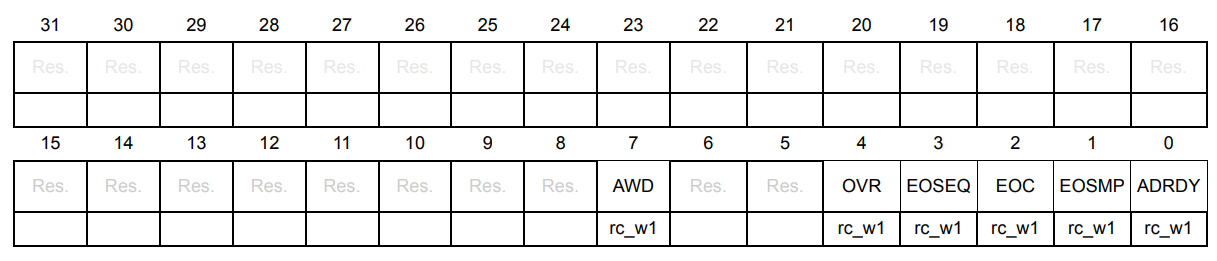
\includegraphics[width=\linewidth]{ADC-ISR-Register.png}
                \caption{ADC-ISR-Register}
                \label{caption:ADC-ISR-Register}
            \end{figure}
             
            \begin{itemize}
                \item EOC (End of conversion):\\
                0: Channel conversion not complete (or the flag event was already acknowledged and cleared by
                software)\\
                1: Channel conversion complete
                \item ADRDY (ADC ready):
                0: ADC not yet ready to start conversion (or the flag event was already acknowledged and cleared
                by software)\\
                1: ADC is ready to start conversion
            \end{itemize}
            
\newpage
        \subsubsection{ADC\_IER | ADC enable Interrupts}
            \begin{figure}[!htb]
                \centering
                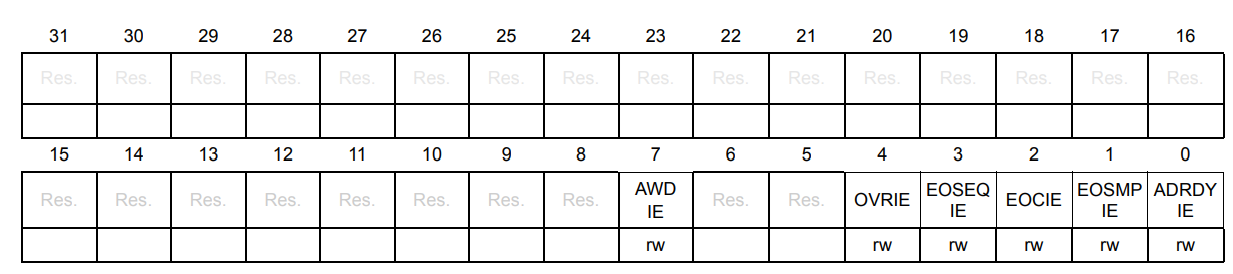
\includegraphics[width=\linewidth]{ADC-IER-Register.png}
                \caption{ADC-IER-Register}
                \label{caption:ADC-IER-Register}
            \end{figure}
            \noindent Benötigt wird:
            \begin{itemize}
                \item EOCIE(End of conversion interrupt enable):\\
                0: EOC interrupt disabled\\
                1: EOC interrupt enabled. An interrupt is generated when the EOC bit is set.
                \item ADRDYIE (ADC ready interrupt enable):
                0: ADRDY interrupt disabled.\\
                1: ADRDY interrupt enabled. An interrupt is generated when the ADRDY bit is set.
            \end{itemize}



        \subsubsection{ADC\_CR | ADC kalibrieren, aktivieren, starten}
            \begin{figure}[!htb]
                \centering
                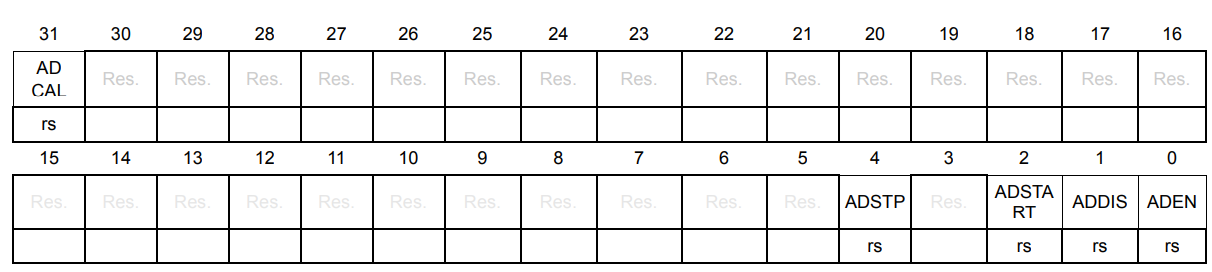
\includegraphics[width=\linewidth]{ADC-CR-Register.png}
                \caption{ADC-CR-Register}
                \label{caption:ADC-CR-Register}
            \end{figure}
            \noindent Benötigt wird:
            \begin{itemize}
                \item ADCAL (ADC calibration):\\
                0: Calibration complete \\
                1: Write 1 to calibrate the ADC. Read at 1 means that a calibration is in progress.
                \item ADEN (ADC enable command)\\
                0: ADC is disabled (OFF state)\\
                1: Write 1 to enable the ADC. 
                \item ADSTART (ADC start conversion command)\\
                0: No ADC conversion is ongoing. \\
                1: Write 1 to start the ADC. Read 1 means that the ADC is operating and may be converting
            \end{itemize}

\newpage
        \subsubsection{ADC\_CFGR2 | Clock Einstellung}
            \begin{figure}[!htb]
                \centering
                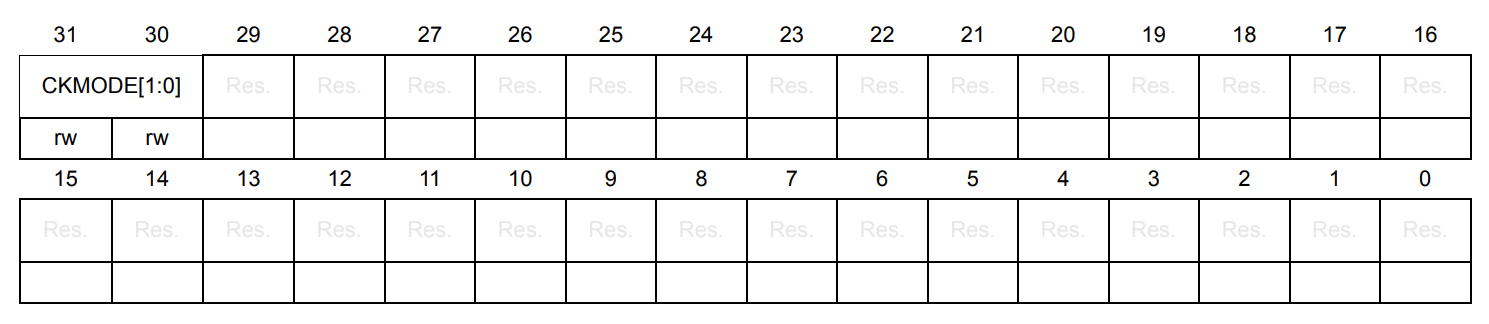
\includegraphics[width=\linewidth]{ADC-CFGR2-Register.png}
                \caption{ADC-CFGR2-Register}
                \label{caption:ADC-CFGR2-Register}
            \end{figure}
            \noindent Benötigt wird:
            \begin{itemize}
                \item CKMODE[1:0] (ADC clock mode):\\
                00: ADCCLK (Asynchronous clock mode), generated at product level (refer to RCC section)\\
                01: PCLK/2 (Synchronous clock mode)\\
                10: PCLK/4 (Synchronous clock mode)\\
                11: Reserved
            \end{itemize}


        \subsubsection{ADC\_CHSELR | ADC Input Channel}
            \begin{figure}[!htb]
                \centering
                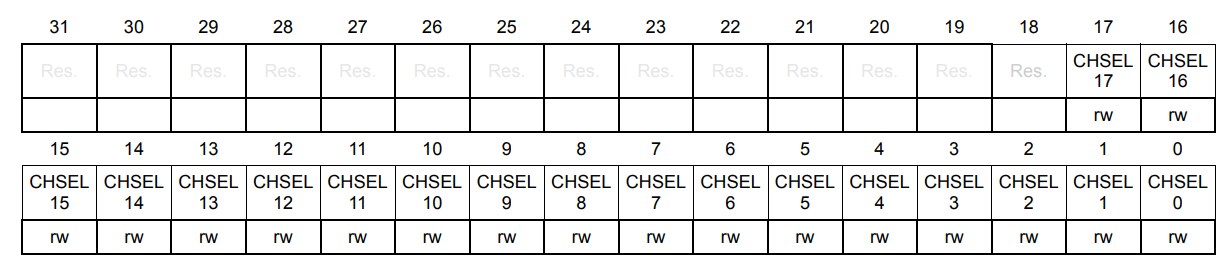
\includegraphics[width=\linewidth]{ADC-CHSELR-Register.png}
                \caption{ADC-CHSELR-Register}
                \label{caption:ADC-CHSELR-Register}
            \end{figure} 
            \noindent Benötigt wird:
            \begin{itemize}
                \item CHSELx: Channel-x selection\\
                0: Input Channel-x is not selected for conversion\\
                1: Input Channel-x is selected for conversion
            \end{itemize}

\newpage
        \subsubsection{ADC\_DR | 16 Bit Ergebniss der Umnwandlung}
            \begin{figure}[!htb]
                \centering
                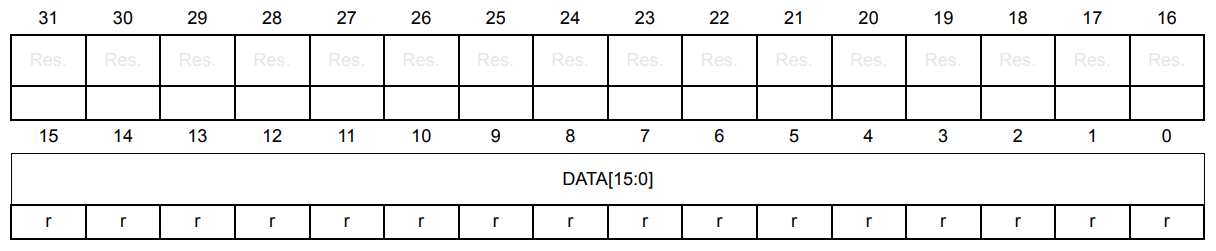
\includegraphics[width=\linewidth]{ADC-DR-Register.png}
                \caption{ADC-DR-Register}
                \label{caption:ADC-DR-Register}
            \end{figure}
            \noindent Benötigt wird:
            \begin{itemize}
                \item DATA[15:0]: Converted data
            \end{itemize}
            
        
        
    
    \subsection{Konfiguration}
        Um den ADC zu konfigurieren, wird zuerst der ADC Clock eingestellt $\rightarrow$ der ADC kalibriert $\rightarrow$  
        ADC aktiviert $\rightarrow$  GPIO als ADC Input einstellen.\\
        Wenn die Kalibrierung fertig ist, ist das ADCAL Bit 0. Dann kann der ADC und Interrupts aktiviert werden und eingestellt werden 
        welcher GPIO Pin als Input verwendet wird. Weiterhin wird der ADC im vortlaufenden (continuous) Modus betrieben, sodass im EOC Interrupt die Umwandlung nicht 
        wieder gestartet werden muss. \\\\
        
        \noindent Danach wenn der ADC bereit ist wird im Interrupt Register die ADC\_ADRDY (ADC Ready) flag gesetzt, dieses wird im ADC-Interrupt-Handler abgefragt und dann
        eine Umwandlung gestartet.\\ 
        Wenn eine Umwandlung fertig ist wird im Interrupt Register das ADC\_TC (Transmission complete) flag gesetzt. Im ADC-Interrupt-Hanlder wird dann aus dem ADC\_DR Register
        das Ergebniss der Umwandlung weitergeben um dies dann an der USART senden zu können.
    
\newpage
    \subsection{ADC-Initiallisierungs-Code}
        \begin{lstlisting}[language=C, style=CStyle, caption=ADC-Initiallisierungs-Code, captionpos=b, label=ADC-Initiallisierungs-Code]
int init_ADC()
{   
    uint32_t reg_content;
    uint32_t* adc_chselr = ADC_CHSELR;
    uint32_t* adc_isr = ADC_ISR;       
    uint32_t* adc_cr = ADC_CR;
    uint32_t* adc_cfgr1 = ADC_CFGR1;
    uint32_t adc_cr_adcal = ADC_CR_ADCAL;
    uint32_t* adc_ier = ADC_IER;
    uint32_t* adc_cfgr2 = ADC_CFGR2;
    uint32_t adc_isr_adrdy = ADC_ISR_ADRDY;
    
    //set ADC clock to PCLK so thats is synchronous with sysclock
    reg_content = *adc_cfgr2;
    reg_content |= 0x40000000;
    *adc_cfgr2 = reg_content;
    //before starting callibrate ADC
    reg_content = *adc_cr;
    reg_content |= adc_cr_adcal;
    *adc_cr = reg_content;

    //if calibration is complete enable ADC
    //enable Interrupts
    //set correct channel
    //when ADC is ready, a ad ready interrupt occurs and the interrupt handler
    //will then start the ADC convertion
    while((*adc_cr & adc_cr_adcal) == adc_cr_adcal); // wait till callibration is complete

    //enable ADC and ensure ADSTART=0 for further configuration and enable ADC
    reg_content = *adc_cr;
    reg_content |= 0x00000001;
    *adc_cr = reg_content;
    //set ADC to continues convertion so, that convertion doesn't to start again in Interrupt
    reg_content = *adc_cr;
    reg_content |= 0x0000200;
    *adc_cr = reg_content;
    //enable Interrupts of ADC
    reg_content = *adc_ier;
    reg_content |= 0x00000005;
    *adc_ier = reg_content;
    //Set ADC Channel to channel 0 because PA0 is ADC_IN0
    reg_content = *adc_chselr;
    reg_content |= 0x00000001;
    *adc_chselr = reg_content;
}
        \end{lstlisting}
\newpage
    \subsection{ADC-Interrupt-Handler-Code}
        \begin{lstlisting}[language=C, style=CStyle, caption=ADC-Interrupt-Handler-Code, captionpos=b, label=ADC-Interrupt-Handler-Code]
void ADC1_IRQHandler(void)   
{
    uint32_t* adc_isr = ADC_ISR;
    uint32_t* adc_cr = ADC_CR;

    uint32_t adc_isr_eoc = ADC_ISR_EOC;
    uint32_t adc_isr_adrdy = ADC_ISR_ADRDY;
    uint32_t* adc_dr = ADC_DR;
    uint32_t adc_dr_data = ADC_DR_DATA;
    uint32_t* gpioa_odr = GPIOA_ODR;
    uint32_t* usart1_tdr =  USART1_TDR;
    
    uint32_t adc_cr_adstart = ADC_CR_ADSTART;
    uint16_t ADC_Value;
    
    uint32_t reg_content;

    //if ADC Ready start convertion
    if((*adc_isr & adc_isr_adrdy) == adc_isr_adrdy)
    {
        reg_content = *adc_cr;
        reg_content |= adc_cr_adstart;
        *adc_cr = reg_content;
    }

    //if convertion complete send ADC value
    if((*adc_isr & adc_isr_eoc) == adc_isr_eoc)
    {
        send=0;
        ADC_Value = (*adc_dr & adc_dr_data);
        //Set PA7 and PA6 high for max to send data
        reg_content = *gpioa_odr;
        reg_content |= 0x000000C0;
        *gpioa_odr = reg_content;
        
        sprintf(USART_write_data, "%d", ADC_Value);
    
        //write something into the USART Buffer for USART
        //interrupt where rest of adc value gets put into the buffer
        *usart1_tdr = 'n'; 
    }
}
        \end{lstlisting}
\newpage
\section{NVIC}
    \subsection{Wir wird er verwendet}
        Beim Programmieren des STM muss der Vector Table beschrieben werden mit einem Assembler File und Linker Skript, diese werden von der Cube IDE erstellt.\\
        Im Vector Table sind alle Interrupts mit dem entsprechenden Funktionnamen für das Programm hinterlegt.
        Im NVIC\_ISER Register können die Interrupts durch ihre Interrupt Position aktiviert werden.\\\\
        Die IRQ\_Handler Positionen werden beim programmieren des uC in den Flash geschrieben. 

        \begin{figure}[!htb]
            \centering
            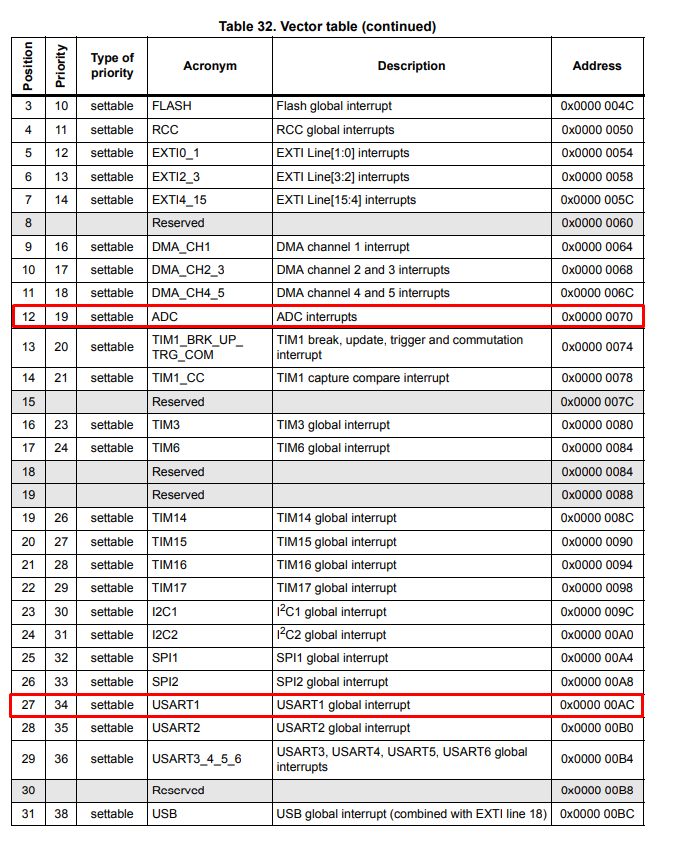
\includegraphics[scale=0.65]{NVIC-Vector-Table.png}
            \caption{NVIC-Vector-Table}
            \label{caption:ANVIC-Vector-Table}
        \end{figure}

\newpage
        \begin{figure}[!htb]
            \centering
            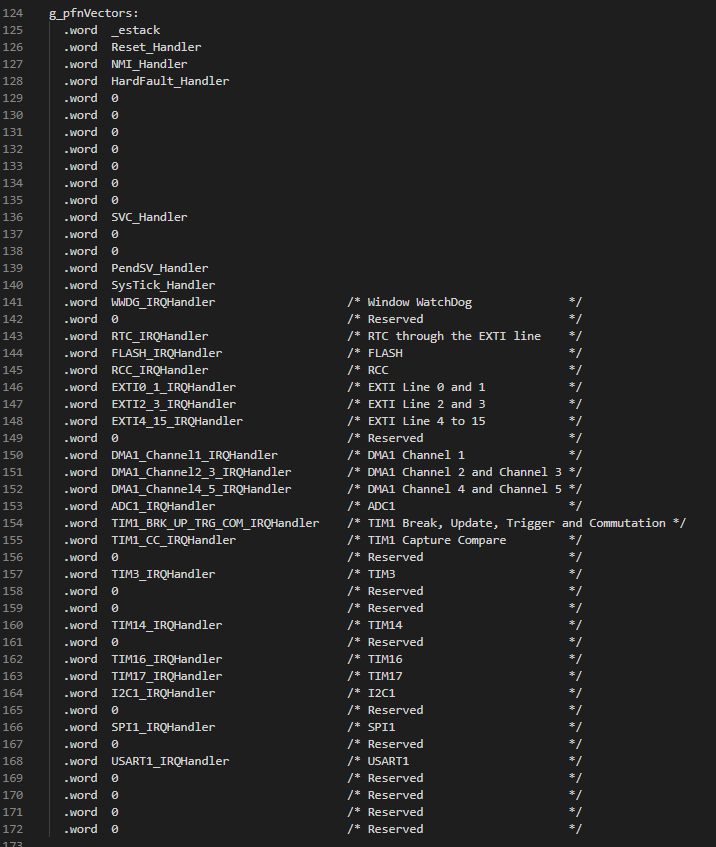
\includegraphics[width=\linewidth]{Ausschnit-Assembler-File.png}
            \caption{Ausschnit-Assembler-File}
            \label{caption:Ausschnit-Assembler-File}
        \end{figure}
\newpage
        \begin{figure}[!htb]
            \centering
            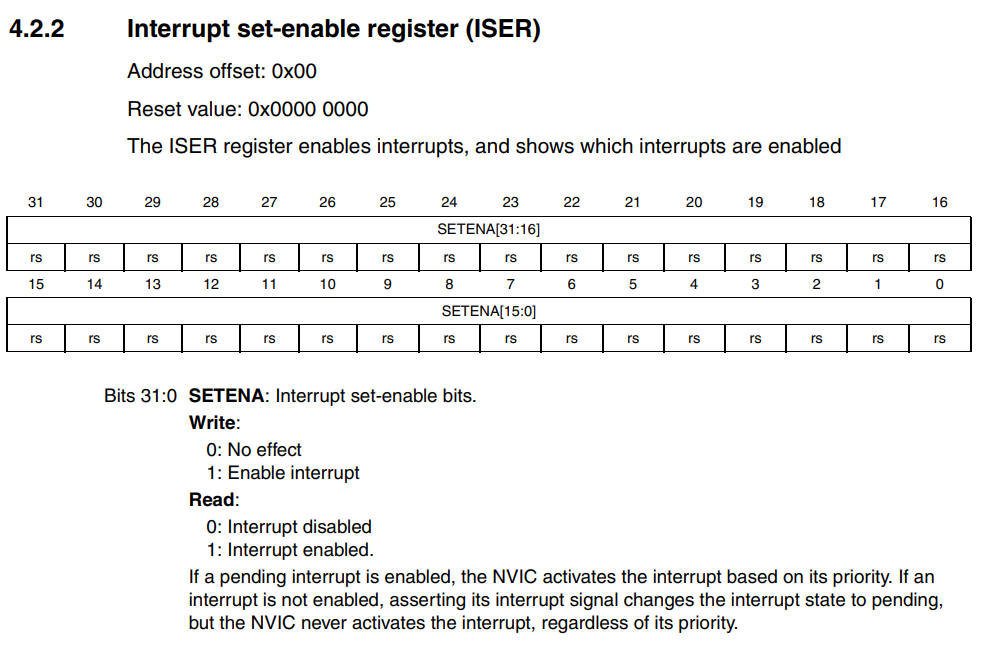
\includegraphics[width=\linewidth]{NVIC-ISER-Register.png}
            \caption{NVIC-ISER-Register}
            \label{caption:NVIC-ISER-Register}
        \end{figure}
        
    \subsection{NVIC-Code}
        \begin{lstlisting}[language=C, style=CStyle, caption=NVIC-enable-interrupts, captionpos=b, label=NVIC-enable-interrupts]
void NVIC_enable_interrupts(void)
{
    uint32_t* nvic_iser =  NVIC_ISER;
    uint32_t reg_content;
    reg_content = *nvic_iser;
    reg_content |= 0x08001000;
    *nvic_iser = reg_content;
}
        \end{lstlisting}

\newpage
\section{Gesamtes-Programm}
\subsection{Headerfile}
\lstinputlisting[language=C, style=CStyle, caption=Headerfile, captionpos=b, label=Headerfile]{../Programm/header.h}
\newpage
\subsection{Main}
\lstinputlisting[language=C, style=CStyle, caption=Gesamter-Code, captionpos=b, label=Gesamter-Code]{../Programm/Programm.c}


\newpage
\section{Anhang}
\subsection{Verlinkungen}
    \begin{tcolorbox}[notitle,boxrule=0pt,colback=gray!20]
        Abbildung: 0\\
        \url{http://www.mathe-mit-methode.com/schlaufuchs_web/elektrotechnik/mikrocontroller_lernmaterial/microcontroller_allgemein/mikrocontroller_ext_hardware/mikrocontroller_uart_bild_001.html} \\
        
        Abbildung: \ref{caption:RS485-Diagramm} 
        \\\url{https://de.wikipedia.org/wiki/EIA-485}\\
        
        Abbildung: \ref{caption:STM32F030F4P6-Pinout}\\
        \href{https://user-images.githubusercontent.com/20950920/48240567-e985c080-e3db-11e8-8775-68a216485b59.jpg}{https://user-images.githubusercontent.com/20950920/48240567-e985c080-e3db-11e8-8775-68a216485b59.jpg}
        von \href{https://github.com/stm32duino/Arduino_Core_STM32/issues/165}{aryeguetta}\\

    \end{tcolorbox}
   
        
%End------------------------------------------------------------------------------------------------------------------------------------------
%---------------------------------------------------------------------------------------------------------------------------------------------
%Codeverzeichnis
\end{document}
